\section{Validation}
\label{sec:validation}
\begin{itemize}
	\item In this section, we use the \bcool specification presented in Listing~\ref{lst:bcoolrunningexample} to coordinate the running example. The application of \bcool operators generates a coordination specification in \ccsl. Figure~\ref{?} shows the partial specification in \ccsl. The specification begins by importing the \ccsl of each models. Then, the coordination is specified by adding some constraints. More precisely, it specifies a simultaneous occurrence between the coordinated events.      
	
	
	 \item The \ccsl specification can be executed by using TimeSquare~\cite{timesquarebib}. Figure~\ref{fig:coffemachinevcd} illustrates the partial timing output of the execution of the running example. TimeSquare also offers the possibility to obtain by exploration quantitative results on the scheduling state-space (see Figure~\ref{?}). The state space is always computable if models are finite. 
	
	 \item \todo{To show the space state}
	  \item \todo{To change the picture, add :}
	\begin{figure}[h]
	  	\center
	  	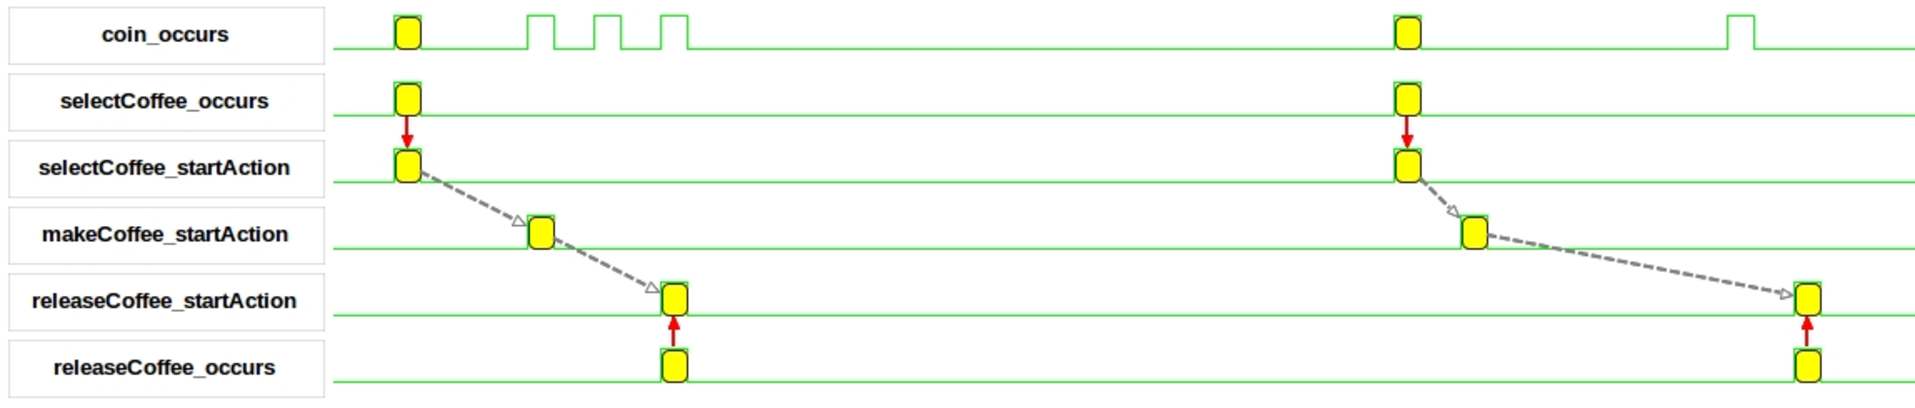
\includegraphics[width=.9\textwidth]{bcool/figs/coffeemachinevcd}
	  	\caption{todo}
	  	\label{fig:coffemachinevcd}
	\end{figure}
	
	\item When a coin is inserted (\emph{coin:occurs} happens), the \emph{selectCoffee:occurs} event is triggered. Then, the coordination forces a simultaneous occurrence between \emph{selectCoffee:occurs} and \emph{selectCoffee:startAction} thus making the activity starts to execute. Then, when the coffee is released, the coordination forces a simultaneous occurrence between the events \emph{releaseCoffee:startAction} and \emph{releaseCoffee:occurs}. The coordination constrains some events by making them to happen simultaneously. This reduces what can be done by individual models, \ie some FSMEvents and Action can only occurs simultaneously. Other events are only constrained by the individual semantics that decides when they occur. The coordination only constraints the behavior of both models without adding new ones. In this sense, the coordination is non intrusive thus not altering the behavior of individual models. 
	
\end{itemize}